\newpage
\section {Билет 6. Транзакции, блокировки, версионность.}


\textbf{Транзакция} — это набор операций в базе данных, которые должны быть либо все выполнены, либо все не выполнены. Транзакции применяются для обеспечения безопасности, верности и непротиворечивости данных в таблице.

\textbf{1 Феномен грязной записи}

Пример: Транзакция T1 модифицирует элемент данных. После этого другая транзакция T2 тоже модифицирует этот элемент данных перед тем, как T1 выполнит COMMITT или ROLLBACK. Если T1 или T2 после этого выполнит ROLLBACK, то становится непонятным, каким должно быть корректное значение элемента.

\textbf{2 Феномен «грязного» чтения (dirty read)}

Транзакция T1 модифицировала содержимое элемента данных. После этого другая транзакция T2 прочитала содержимое этого элемента данных, до того как транзакция T1 выполнила операцию COMMIT (зафиксировалась) или ROLLBACK (откатилась). Если T1 завершается операцией ROLLBACK, то получается, что транзакция T2 прочитала реально не существующие данные.


\textbf{2.5 Феномен потерянной модификации}

Аномалия потерянной модификации происходит в случае, когда транзакция T1 прочитала элементы данных, после нее T2 их модифицировала (возможно, исходя из предыдущего чтения), после чего T1 (основываясь на ранее прочитанном ею значении) модифицирует содержимое элемента данных и фиксируется.

\textbf{3 Феномен неповторяемого чтения (unrepeatable read)}

Транзакция T1 прочитала содержимое элемента данных. После этого другая транзакция T2 модифицирует или удаляет этот элемент данных и фиксируется. Если T1 после этого попытается прочитать содержимое этого элемента данных снова (она еще не завершилась), то она получит другое значение или обнаружит, что элемент данных больше не существует.

\textbf{4 Феномен фантомов}

Транзакция T1 прочитала содержимое нескольких элементов данных, удовлетворяющих некоторому предикату . После этого транзакция T2 создает элемент данных, удовлетворяющий этому предикату, и фиксируется. Если транзакция T1 повторит чтение с тем же предикатом , то получит уже другой набор данных, отличный от полученного в первый раз.

Первый способ решения феноменов - \textbf{блокировки}: запрещается доступ к строкам (а может и ко всей таблице) по определенным условиям. Блокировки бывают длинные (до конца транзакций) и короткие (на время выполнения операции). Блокировки на несколько операций не выставляются. 

В таблице показано какие блокировки решают феномены:

\begin{center}
	\begin{tabular}{c|c c}
		Феномен & Чтение & Запись \\
		1 & - & Д \\
		2 & К & Д\\
		3 & Д на курсор & Д \\
		4 & Д на предикат & Д\\
	\end{tabular}
\end{center}

Можно было бы выбрать 3 уровень и радоваться, но нет - будет очень много заблокированных данных. Блокировки уже мало где используются. 
\\[20pt]
\textbf{Версионность.} 

Мы продолжаем выставлять блокировки на запись, но при чтении мы не блокируем запись, а запоминаем в какой момент произвели чтение. 

Пусть есть блок b и ему прописано время 1. В момент времени 1 мы начали выполнять SELECT, который когда-нибудь дойдет до блока b. В момент времени 2 мы переписали значение блока b. Тогда (после изменения данных блока) b приписывается время 2, а часть блока уезжает в сегмент отката. Когда транзакция доходит до блока b, она видит, что у него время 2 (позже ее начала) и идет в сегмент отката за нужными записями. 

\begin{figure}[H]
	\centering
	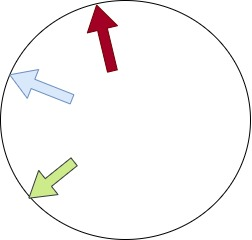
\includegraphics[scale = 0.5]{6/vers.jpg}
	\caption{Сегмент отката}
	\label{fig:vers}
	
\end{figure}

На рисунке \ref{fig:vers} изображена структура сегмента отката. Голубым изображен хвост, а зеленым голова. Голова начинает догонять свой хвост. Но когда мы говорим COMMIT мы передвигаем хвост на последнюю незакоммиченную транзакцию. Если хвост указывает на временную метку 4, голова на 10, а наш запрос пытается получить данные за первый (1) момент времени (показано красной стрелочкой), то произойдет ошибка (снимок слишком старый). Если голова дойдет до хвоста, то будет фатальная ошибка у всех пользователей. 


Журнал версионности также служит способом восстановления бд. Если писать изменения данных сразу на диск, то бд будет работать супер долго. Просто в памяти хранить нельзя (можем потерять все изменения даже если были коммиты). Однако, можно писать на диск журнал изменений. Туда пишутся только сами изменения (это весит гораздо меньше) и мы говорим пользователю, что все сохранили, только если журнал изменений записался на диск. 
\\[20pt]
\textbf{Простейший пример взаимной блокировки (deadlock):}

\begin{center}
	\begin{tabular}{c|c | c}
		Шаг	& Процесс 1	& Процесс 2 \\
		0	&Хочет захватить A и B, начинает с A &	Хочет захватить A и B, начинает с B \\
		1&	Захватывает ресурс A &	Захватывает ресурс B \\
		2&	Ожидает освобождения ресурса B	& Ожидает освобождения ресурса A \\
		3	&Взаимная блокировка & Взаимная блокировка
	\end{tabular}
\end{center}

Для решения такой проблемв просто кого-то вышибают (отклоняют операцию) - это простое решение проблемы. Сложнее обнаружить такую ситуацию, для этого используют поиск циклов в графе. Пример такого цикла на Рис.\ref{fig:dead}. R - ресурс, P - процесс. 

\begin{figure}[H]
	\centering
	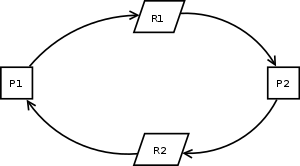
\includegraphics[scale = 0.5]{6/deadlock.png}
	\caption{Граф deadlock}
	\label{fig:dead}
	
\end{figure}
